% Provenance (never printed): the money strand of ../economics_series.md (grade 7). Brief: sources/book1/BRIEFS.md,
% g7-04. Chart data: figdata/grade-7/04-money (WDI FX.OWN.TOTL.ZS, from the Global Findex survey; barter-rate counts).
% Ledger: g7:radford-1945, g7:radford-issue, g7:radford-bread, g7:lydian-coin-date.
\chapter{Money}\label{ch:g7:money}

\begin{openingchart}{Share of adults with an account at a bank, another financial
institution or a mobile-money provider, in 2011 and in 2024, in ten countries and in
the whole world.}{World Bank, World Development Indicators, FX.OWN.TOTL.ZS (Global
Findex survey), 2011 and 2024}
\begin{tikzpicture}
\begin{axis}[omrecord, xbar, bar width=5pt, xmin=0, xmax=100, grid=none, xmajorgrids,
  ytick=data, yticklabels from table={figdata/grade-7/04-money/out/accounts.csv}{label},
  y tick label style={font=\footnotesize}, enlarge y limits=0.06,
  xlabel={Percent of adults (aged 15 and over)}, height=0.62\linewidth,
  legend style={at={(0.5,-0.14)}, anchor=north, legend columns=2}, reverse legend]
\addplot[fill=omExo!45, draw=omExo] table[y=pos, x=y2011] {figdata/grade-7/04-money/out/accounts.csv};
\addplot[fill=omMeth!60, draw=omMeth] table[y=pos, x=y2024] {figdata/grade-7/04-money/out/accounts.csv};
\legend{2011, 2024}
\end{axis}
\end{tikzpicture}
\end{openingchart}

% figdata: accounts (EGY 9.7 43.1; PAK 10.3 27.3; KEN 42.3 90.1; IND 35.2 89.0; GHA 29.4 81.2; WLD 50.6 78.7;
% CHN 63.8 89.4)
In 2011, half of the world's adults ($50.6\,\%$) had an account in which to keep \omterm{def:g7:money:money}{money}
and from which to pay. In 2024, $78.7\,\%$ did. In Kenya the share went from $42.3\,\%$
to $90.1\,\%$, in India from $35.2\,\%$ to $89.0\,\%$, often through a phone: a
\omterm{def:g7:money:money}{mobile-money} account lets its owner pay a shop or send \omterm{def:g7:money:money}{money} to a relative with a text
message. In Pakistan, the share was still $27.3\,\%$ in 2024.

\begin{dated}{2026}
% figdata: accounts (WLD 2011 50.6, 2024 78.7)
The latest survey of accounts was made in 2024: $78.7\,\%$ of the world's adults had an
account. The next survey will change these numbers.
\end{dated}

Coins, notes, a number in an account, a payment by phone: all are \omterm{def:g7:money:money}{money}. This chapter
asks what \omterm{def:g7:money:money}{money} does, why people use it rather than swapping goods, and what makes some
things good \omterm{def:g7:money:money}{money} and others bad.

\begin{recall}
In an exchange, each side gives something to the other (\cref{ch:g7:specialisation}).
\omterm{def:g7:specialisation:specialisation}{Specialisation} and exchange bring \omterm{def:g7:comparative-advantage:gains-from-trade}{gains from trade}
(\cref{ch:g7:comparative-advantage}).
\end{recall}

\section{Barter}

\begin{definition}[Barter]\label{def:g7:money:barter}
\emph{Barter}\index{barter} is the exchange of goods or services directly for other
goods or services, without \omterm{def:g7:money:money}{money}.
\end{definition}

\begin{omfigure}
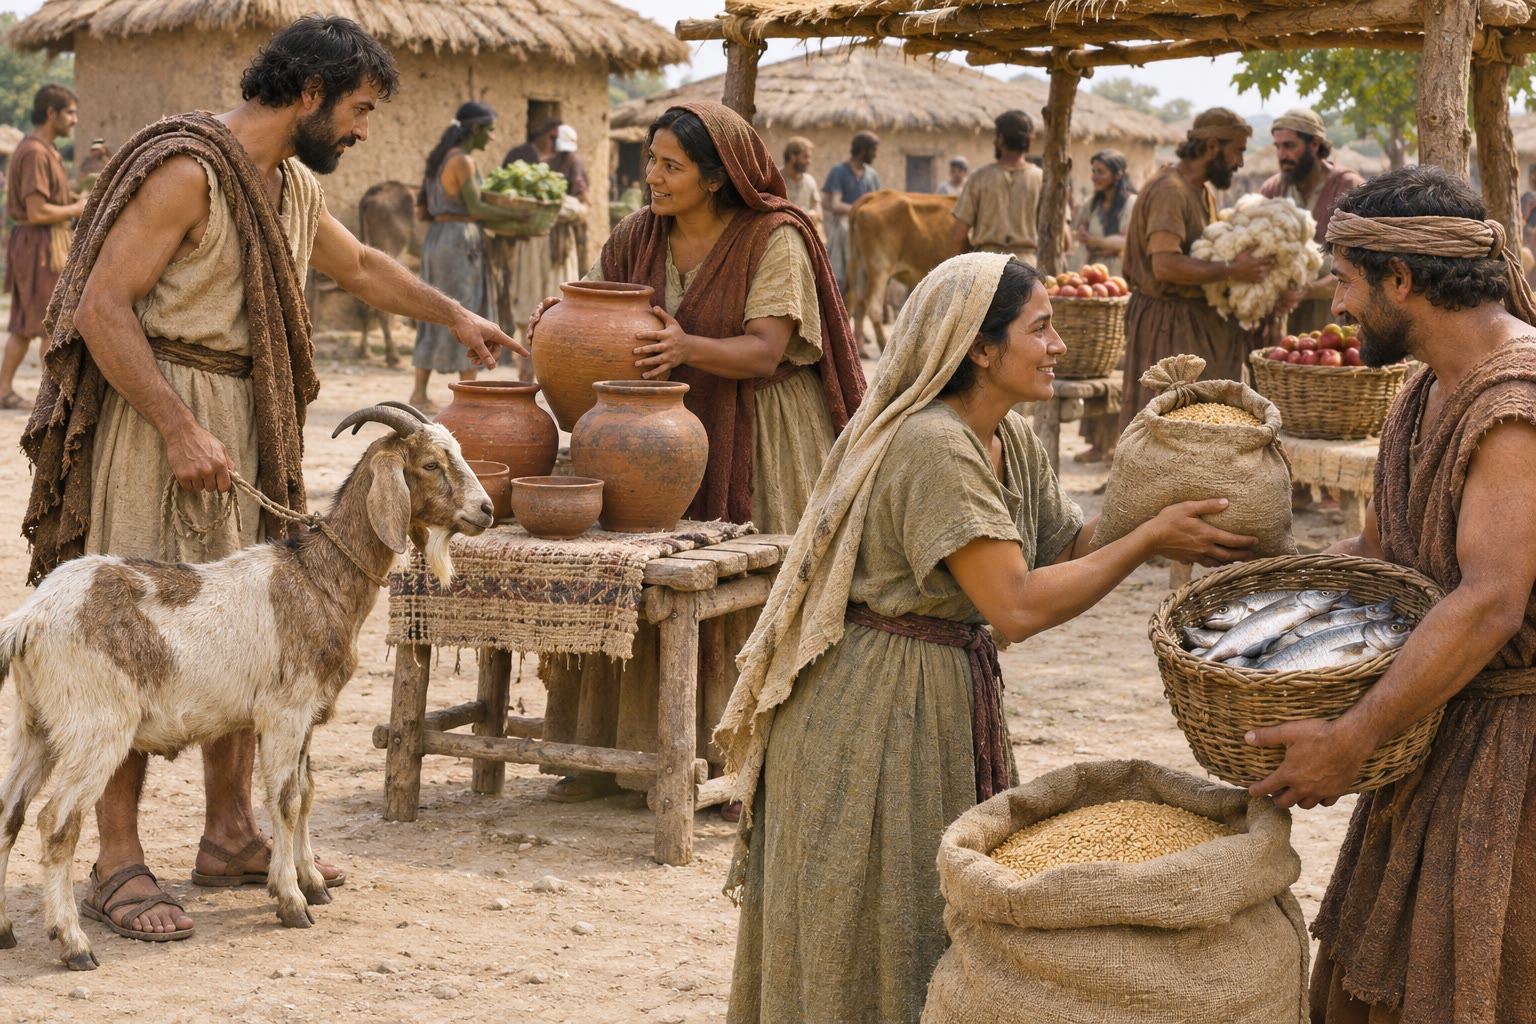
\includegraphics[width=0.55\linewidth]{images/book1/ai/g7-money-barter-market.jpg}

{\small A \omterm{def:g7:money:barter}{barter} market: a goat for pots, grain for fish. Every exchange needs two people
who each want what the other has.}
\end{omfigure}

\omterm{def:g7:money:barter}{Barter} works between neighbours who know each other's needs. It works badly in a large
market, for a simple reason.

\begin{definition}[Double coincidence of wants]\label{def:g7:money:double-coincidence}
A \emph{double coincidence of wants}\index{double coincidence of wants} is the situation
in which each of two people has what the other wants and wants what the other has.
\omterm{def:g7:money:barter}{Barter} needs one for every exchange.
\end{definition}

\begin{omfigure}
\begin{tikzpicture}[econ, x=1cm, y=1cm,
  tr/.style={draw, rounded corners=2pt, fill=omMeth!12, align=center, font=\scriptsize,
    minimum width=2.3cm, minimum height=1cm}]
  \begin{scope}
    \node[tr] (a) at (90:2.3) {Ali has fish\\wants grain};
    \node[tr] (b) at (210:2.3) {Bea has grain\\wants pots};
    \node[tr] (c) at (330:2.3) {Cem has pots\\wants fish};
    \draw[-{Stealth}, thick, omExo] (a) to[bend right=20] node[left, font=\scriptsize] {wants} (b);
    \draw[-{Stealth}, thick, omExo] (b) to[bend right=20] node[below, font=\scriptsize] {wants} (c);
    \draw[-{Stealth}, thick, omExo] (c) to[bend right=20] node[right, font=\scriptsize] {wants} (a);
    \node[font=\footnotesize] at (0,-2.45) {barter: no pair can trade};
  \end{scope}
  \begin{scope}[xshift=7.6cm]
    \node[tr] (a2) at (90:2.3) {Ali};
    \node[tr] (b2) at (210:2.3) {Bea};
    \node[tr] (c2) at (330:2.3) {Cem};
    \node[draw, circle, fill=omDef!25, font=\scriptsize, align=center] (m) at (0,0) {money};
    \draw[{Stealth}-{Stealth}, thick, omMeth] (a2) -- (m);
    \draw[{Stealth}-{Stealth}, thick, omMeth] (b2) -- (m);
    \draw[{Stealth}-{Stealth}, thick, omMeth] (c2) -- (m);
    \node[font=\footnotesize] at (0,-2.45) {money: each sells and buys};
  \end{scope}
\end{tikzpicture}

{\small Three invented traders. Each wants what the next one has, so no two of them can
\omterm{def:g7:money:barter}{barter}. With \omterm{def:g7:money:money}{money}, Ali sells fish to Cem, buys grain from Bea, and each gets what he or
she wants.}
\end{omfigure}

A second difficulty is the number of \omterm{def:g7:money:price}{prices}. With 4 goods, \omterm{def:g7:money:barter}{barter} needs a rate for each
pair of goods: fish for grain, fish for pots, fish for cloth, grain for pots, grain for
cloth, pots for cloth --- 6 rates. With \omterm{def:g7:money:money}{money}, 4 \omterm{def:g7:money:price}{prices} are enough, one per good. With
10 goods, \omterm{def:g7:money:barter}{barter} needs 45 rates; \omterm{def:g7:money:money}{money}, 10 \omterm{def:g7:money:price}{prices}.
% figdata: barter (4: 6 rates; 10: 45 rates)

\section{What money does}

\begin{definition}[Money]\label{def:g7:money:money}
\emph{Money}\index{money} is anything that is widely accepted in a society as payment
for goods and services and for the settling of debts.
\end{definition}

\omterm{def:g7:money:money}{Money} does three jobs.

\begin{definition}[Means of payment]\label{def:g7:money:means-of-payment}
\omterm{def:g7:money:money}{Money} is a \emph{means of payment}\index{means of payment}: it is given in exchange for
goods and services, and accepted because others will accept it in turn.
\end{definition}

\begin{definition}[Unit of account]\label{def:g7:money:unit-of-account}
\omterm{def:g7:money:money}{Money} is a \emph{unit of account}\index{unit of account}: \omterm{def:g7:money:price}{prices}, wages, debts and
budgets are all written in it, so that they can be compared and added.
\end{definition}

\begin{definition}[Store of value]\label{def:g7:money:store-of-value}
\omterm{def:g7:money:money}{Money} is a \emph{store of value}\index{store of value}: it can be kept today and spent
later, and still buy roughly as much.
\end{definition}

\begin{measure}[An account]
The chart that opens the chapter counts the adults who answered ``yes'' in a survey made in
each country: do you, alone or with someone else, have an account at a
bank or another financial institution, or use a \omterm{def:g7:money:money}{mobile-money} service? An account is a
record of \omterm{def:g7:money:money}{money} that its owner can pay from; the survey does not ask how much is in it
or how often it is used.
\end{measure}

\section{What has served as money}

Many things have served as \omterm{def:g7:money:money}{money}: cattle, grain, salt, shells, beads, pieces of metal by
weight, then coins, notes printed on paper, and today numbers in accounts. Coins were a
great step, because a ruler's mark promised the weight and the metal: nobody had to weigh
and test each piece.

\begin{omfigure}
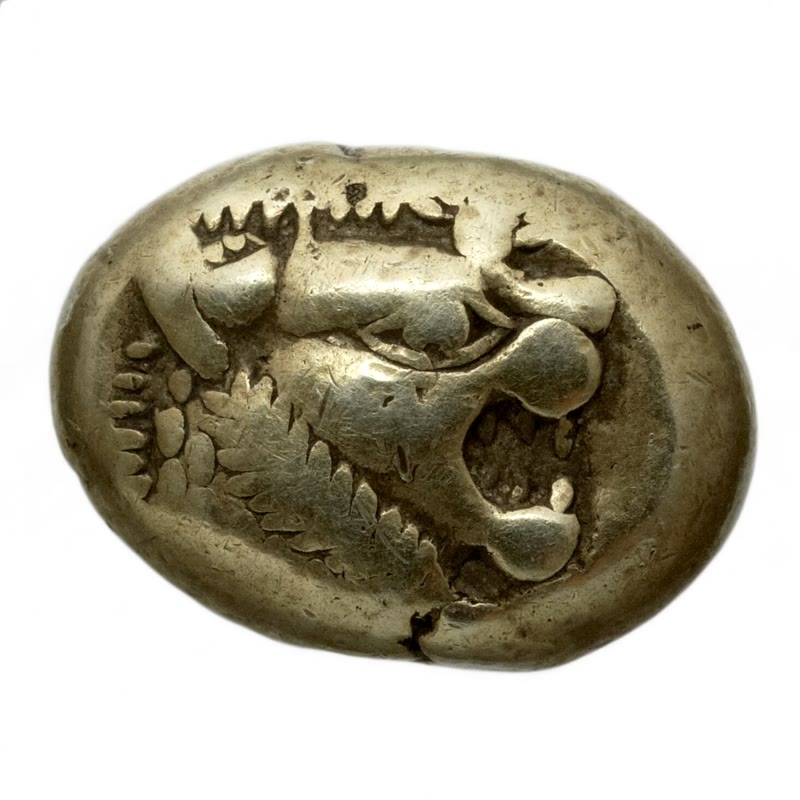
\includegraphics[width=0.38\linewidth]{images/book1/photos/g7-money-lydian-electrum-trite.jpg}

{\small An electrum coin (a natural mix of gold and silver) struck in Lydia, in the west of
today's Turkey. Coins of this kind are dated to about 600--530 before the common era. The
lion's head is the mark of the issuer.}
% ledger: g7:lydian-coin-date
\end{omfigure}

\begin{record}[Cigarettes as money]
% ledger: g7:radford-1945, g7:radford-issue, g7:radford-bread
During the Second World War, prisoners in a camp received food and cigarettes in parcels
from the Red Cross, among them 25 or 50 cigarettes per man per week. They began to swap
food and cigarettes, and cigarettes soon became the camp's \omterm{def:g7:money:money}{money}: \omterm{def:g7:money:price}{prices} were written in
cigarettes, goods were sold for them, and they were saved. A bread ration cost about 7
cigarettes, rising to 8 before the next issue came. Cigarettes were all alike, kept well
and could pay for small or, in packets, large purchases. But cigarettes were also smoked:
when parcels stopped coming, the stock of cigarettes shrank, \omterm{def:g7:money:price}{prices} in cigarettes fell and
trading turned back to \omterm{def:g7:money:barter}{barter}; when a large delivery arrived, \omterm{def:g7:money:price}{prices} shot up. No one had
designed this \omterm{def:g7:money:money}{money}; the prisoners chose it because it worked (Radford, 1945).
\end{record}

\section{What makes good money}

The cigarettes of the camp show what a good \omterm{def:g7:money:money}{money} needs:
\begin{itemize}
  \item \textbf{Accepted}: everyone takes it, because everyone else does.
  \item \textbf{Durable}: it does not rot, break or wear out quickly.
  \item \textbf{Divisible}: it can pay for small and large things.
  \item \textbf{Hard to forge}: false pieces are rare, so it need not be checked each time.
  \item \textbf{Scarce, but not too scarce}: its quantity does not jump up or down, so its
        value stays steady.
\end{itemize}
Fish fail on durability, cattle on divisibility, cigarettes on steadiness (they were
smoked). The notes and accounts of today are not valuable in themselves; they work because
they are accepted and their quantity is controlled, as later chapters explain.

\begin{model}{Money as a means of exchange}
\assumes Trading is costly without a common good that everyone accepts; people want to
save the time spent searching for a \omterm{def:g7:money:double-coincidence}{double coincidence of wants}.
\predicts One widely accepted, durable and divisible good comes to serve as \omterm{def:g7:money:money}{money}; a
society that loses its \omterm{def:g7:money:money}{money} turns back to \omterm{def:g7:money:barter}{barter} or adopts another good as \omterm{def:g7:money:money}{money}.
\tested Cigarettes became the \omterm{def:g7:money:money}{money} of a prisoner-of-war camp, and trading turned back to
\omterm{def:g7:money:barter}{barter} when they ran short (the record above).
\breaks \omterm{def:g7:money:money}{Money} whose value falls fast stops being a \omterm{def:g7:money:store-of-value}{store of value}: people then spend it at
once or switch to another \omterm{def:g7:money:money}{money} (\cref{ch:g8:inflation-and-price-indices}).
\end{model}

\section{A price is an amount of money}

\begin{definition}[Price]\label{def:g7:money:price}
The \emph{price}\index{price} of a good is the amount of \omterm{def:g7:money:money}{money} that must be given for one
unit of it.
\end{definition}

A \omterm{def:g7:money:price}{price} compares a good with \omterm{def:g7:money:money}{money}, and so, through \omterm{def:g7:money:money}{money}, with every other good. If a
loaf costs 2 dalens and a shirt 30 dalens, a shirt is worth 15 loaves. If every \omterm{def:g7:money:price}{price} and
every wage were doubled at once, nothing real would change: a shirt would still be worth
15 loaves and an hour of work would buy as much as before. What matters for a buyer is a
\omterm{def:g7:money:price}{price} compared with other \omterm{def:g7:money:price}{prices} and with income.

\section{Exercises}

\begin{exercise}[$\star$]\label{exo:g7:money:1}
Use the opening chart. About what share of adults had an account in Nigeria in 2011, and
in 2024?
\end{exercise}

\begin{exercise}[$\star$]\label{exo:g7:money:2}
A \omterm{def:g7:money:barter}{barter} market has 4 goods: fish, grain, pots and cloth. (a) List all the pairs of goods
that need an exchange rate. How many are there? (b) How many \omterm{def:g7:money:price}{prices} are needed with \omterm{def:g7:money:money}{money}?
\end{exercise}

\begin{exercise}[$\star$]\label{exo:g7:money:3}
Which job of \omterm{def:g7:money:money}{money} is used in each scene? (a) A café writes its \omterm{def:g7:money:price}{prices} on a board. (b) A
girl puts 5 dalens of her pocket \omterm{def:g7:money:money}{money} in a box for the summer. (c) A man pays for his
bread.
\end{exercise}

\begin{exercise}[$\star$]\label{exo:g7:money:4}
A shop's list gives: bread 2 dalens, milk 1.5 dalens, cheese 6 dalens. Write each \omterm{def:g7:money:price}{price} in
loaves of bread.
\end{exercise}

\begin{exercise}[$\star\star$]\label{exo:g7:money:5}
How many \omterm{def:g7:money:barter}{barter} exchange rates are needed for 10 goods? Explain how you count them.
\end{exercise}

\begin{exercise}[$\star\star$]\label{exo:g7:money:6}
In an invented camp, a bread ration costs 8 cigarettes and a tin of jam 12 cigarettes. A
newcomer measures \omterm{def:g7:money:price}{prices} in dalens and knows that one cigarette is worth 0.25 dalen.
(a) Write both \omterm{def:g7:money:price}{prices} in dalens. (b) How many bread rations is a tin of jam worth? (c) Does
the answer to (b) depend on the unit used?
\end{exercise}

\begin{exercise}[$\star\star$]\label{exo:g7:money:7}
An invented \omterm{def:g7:money:money}{money} loses half of its value every month: what it buys in one month, it buys
only half of the month after. (a) What does a sum that buys 80 loaves today buy after 3
months? (b) Which job of \omterm{def:g7:money:money}{money} does it fail? (c) What would people do with their \omterm{def:g7:money:money}{money}?
\end{exercise}

\begin{exercise}[$\star\star$]\label{exo:g7:money:8}
Use the values in the text. By how many percentage points did the share of adults with an
account rise from 2011 to 2024 in Kenya, and in the world?
\end{exercise}

\begin{exercise}[$\star\star$]\label{exo:g7:money:9}
Describe an observation that would contradict the model ``\omterm{def:g7:money:money}{Money} as a means of exchange''.
\end{exercise}

\begin{exercise}[$\star\star\star$]\label{exo:g7:money:10}
(a) Complete the table of \omterm{def:g7:money:barter}{barter} exchange rates for 2, 3, 4, 5 and 6 goods. (b) Find the
pattern: how many rates does each extra good add? (c) Use it to find the number of rates
for 12 goods.
\end{exercise}

\begin{exercise}[$\star\star\star$]\label{exo:g7:money:11}
In an invented country, forged coins spread and one coin in four is false. Checking a coin
takes a minute. (a) What happens to the time a shopkeeper spends on each sale? (b) What
might people start to use instead of coins? (c) Which property of good \omterm{def:g7:money:money}{money} has been
lost?
\end{exercise}

\begin{exercise}[$\star\star\star$]\label{exo:g7:money:12}
The opening chart counts adults with an account. Name two questions about how people pay
that the chart cannot answer, and say what data would answer one of them.
\end{exercise}

\section{Problem: The Island Market}

\begin{problem}[{Weekend problem --- barter between five traders, shells as money, and the
prices after a find of shells}]
\label{pb:g7:money:1}
Everything in this problem is invented. On a small island, five traders meet each week.
Each has one good and wants another:
\begin{center}
\begin{tabular}{lll}
\toprule
Trader & Has & Wants \\
\midrule
Ana & fish & bread \\
Bo & bread & rope \\
Cy & rope & pots \\
Di & pots & salt \\
Eli & salt & fish \\
\bottomrule
\end{tabular}
\end{center}

\medskip
\noindent\textbf{Part I --- Barter.}
\begin{enumerate}
  \item Can any two traders \omterm{def:g7:money:barter}{barter} directly? Check each pair.
  \item How many \omterm{def:g7:money:barter}{barter} exchange rates would the 5 goods need?
  \item Ana could swap her fish for something she does not want, hoping to swap it again.
        Describe a chain of swaps that brings her bread. How many swaps does it take?
\end{enumerate}

\medskip
\noindent\textbf{Part II --- Shells as money.} The islanders agree to use a rare kind of shell
as \omterm{def:g7:money:money}{money}. The 5 traders hold 100 shells in all. \omterm{def:g7:money:price}{Prices} are: fish 4 shells, bread 2, rope 5,
pots 8, salt 1.
\begin{enumerate}[resume]
  \item How many \omterm{def:g7:money:price}{prices} are needed now?
  \item Ana sells her fish and buys bread. How many shells does she have left over?
  \item Write the \omterm{def:g7:money:price}{price} of a pot in loaves of bread, and the \omterm{def:g7:money:price}{price} of rope in units of salt.
  \item Which jobs of \omterm{def:g7:money:money}{money} do the shells do when (a) Ana writes her \omterm{def:g7:money:price}{prices} on a slate,
        (b) Bo keeps 10 shells for the winter?
  \item Why is it important that the shells are rare and hard to copy?
\end{enumerate}

\medskip
\noindent\textbf{Part III --- A find of shells.} A storm throws a bank of the same shells onto
the beach. The traders collect 100 more: there are now 200 shells, and the goods are the
same.
\begin{enumerate}[resume]
  \item If every \omterm{def:g7:money:price}{price} changes in proportion to the number of shells, what are the new
        \omterm{def:g7:money:price}{prices}?
  \item What is the \omterm{def:g7:money:price}{price} of a pot in loaves of bread now? Compare with question 6.
  \item Bo had saved 10 shells for the winter. What could they buy in bread before the
        storm, and after?
  \item Who gains and who loses from the find of shells?
\end{enumerate}
\end{problem}
